%%%%%%%%%%%%%%%%%%%%%%%%%%%%%%%%%%%%%%%%%%%%%%%%%%%%%%%%%%%%%%%%%%%%%%%%%%%%%%
%% Example thesis LaTeX document using the fsthesis class
%%
%% Compile with pdflatex
%% However there is option that requires LuaLaTex in the class definition file
%%

\documentclass{fsthesis}

\usepackage{lettrine}   % \lettrine{F}{irst}
\usepackage{titlesec}
\usepackage{graphicx}
\usepackage{natbib}
\usepackage{listings}
\usepackage[acronym,toc,nomain]{glossaries}

% Installed
% texlive-luatex
% texlive-latex-recommended
%   fontspec
% texlive-latex-extra
%   lettrine

% Create the acronyms using a seperate file of definitions
\makeglossaries
%% Acronym definitions for thesis


\newacronym{bob}{BOB}{Bob Over Board}
\newacronym{FAAM}{FAAM}{Facility for Airborne Atmospheric Measurements}
\newacronym{WACL}{WACL}{Wolfson Atmospheric Chemistry Laboratories}


\includeonly{thesis_example_chapter}

\begin{document}
\frontmatter
% Create the titlepage
\title{This is my Thesis\\ \& it's very good...}
\author{Fred Fred}				% author
%\degree{Diploma}				% defaults to 'PhD'
%\university{University of Life}% defaults to 'University of York'
%\dept{School of Hard Knocks}	% defaults to 'Department of Chemistry'
\date{\today}%May 2018}         % standard LaTeX \date behaviour
\maketitle

\tableofcontents
%\pagebreak

\mainmatter


\chapter[Testing chapter]{This is a test chapter and so has areally long title}

\typeout{****}
\typeout{chaptername is \chaptername}
\typeout{textwidth is \the\textwidth}
\typeout{chapboxlength is \the\chapboxlength}
\typeout{chaptitlelength is \the\chaptitlelength}
\typeout{****}

\lettrine{Q}{uam} at parturient a diam ultricies nec phasellus augue scelerisque nec tortor a fringilla a a ullamcorper est ultrices mattis a. Consectetur ac ligula at in adipiscing ad sagittis diam quis scelerisque a mauris etiam dignissim mus enim leo. Per congue \textbf{semper nisl nisl mi scelerisque} porta parturient dignissim ad consectetur \textit{scelerisque cubilia vulputate ante} parturient et eu leo. \textsf{Dis mi euismod lacus pulvinar} curae tortor condimentum mattis enim. \textsc{Condimentum fringilla vestibulum aliquam} elit lobortis mi a ut egestas augue a nunc mollis ultrices. Nec at mollis nostra ullamcorper nam leo commodo cursus adipiscing adipiscing blandit per ut a curae vel eleifend adipiscing vitae justo convallis. This here is a really long URL~\citep{url-01}; \url{https://www.long-long-long-long-long-long.com/long-long-long-long-long-long.html}.

\section{Introduction}
Sit vitae montes dictumst quam \acrfull{WACL} ipsum neque consectetur non litora nisl amet et venenatis egestas ad. Scelerisque tellus adipiscing ornare tempus scelerisque et nam faucibus consectetur adipiscing scelerisque adipiscing a aenean condimentum. Vestibulum \acrshort{WACL} vestibulum \acrfull{FAAM} integer fermentum nam tristique a proin accumsan posuere parturient iaculis parturient aliquam lacinia a sagittis curae condimentum convallis. Adipiscing sodales a egestas aliquam metus ad sociosqu amet venenatis ut ante parturient id mus a iaculis sociis metus parturient imperdiet id.
\par
\begin{figure}
\centering
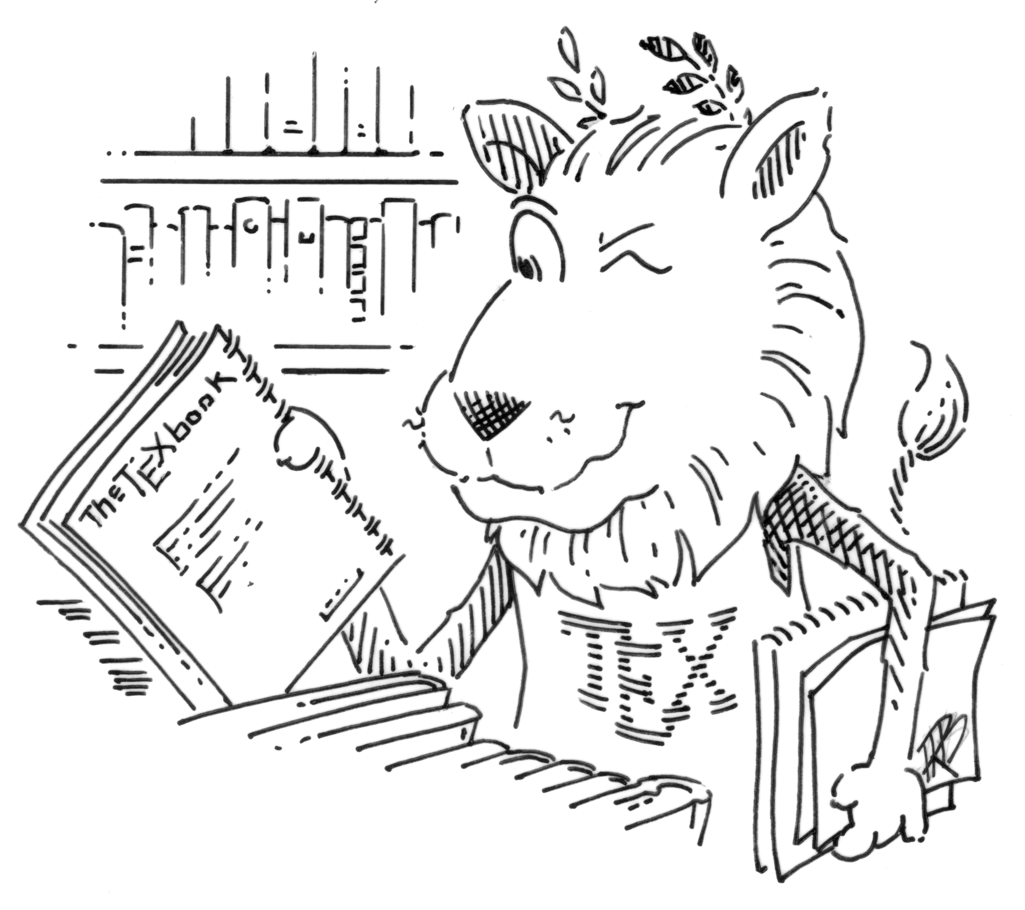
\includegraphics[width=0.5\textwidth]{ctan_lion}
\caption[Short caption of lion]{CTAN lion drawing by Duane Bibby. Integer fermentum nam tristique a proin accumsan posuere parturient iaculis parturient aliquam lacinia a sagittis curae condimentum convallis. Adipiscing sodales a egestas aliquam metus ad sociosqu}
\label{fig:lion}
\end{figure}
{\fontsize{20}{25}\selectfont Auctor a ut ut inceptos parturient} torquent metus condimentum a non risus \acrlong{WACL} eu rhoncus consectetur phasellus ultricies arcu sit nunc condimentum nunc amet tristique erat eu ridiculus. Phasellus elementum massa ridiculus \acrfullpl{bob} ultrices congue nascetur rhoncus eros a sagittis varius aenean cras egestas eu a augue laoreet cum cras phasellus eget hac nostra. \acrshort{bob} in vestibulum porta sapien scelerisque a suspendisse penatibus augue sodales donec egestas adipiscing vitae platea semper urna parturient cubilia, see~\ref{fig:lion}, phasellus donec id mauris a lorem a pretium parturient dictumst.
\par
Lorem ipsum dolor sit amet, consectetur adipiscing elit. Donec molestie tempus nibh ut consectetur. Nunc imperdiet porta urna id porta. Aliquam quis consectetur est. Suspendisse sit amet mattis diam, vel bibendum dolor. Sed vitae est nec leo hendrerit convallis id eu ipsum. Suspendisse lectus justo, scelerisque id interdum in, egestas nec erat. Pellentesque imperdiet sapien quis neque porttitor, quis lobortis ex bibendum. Class aptent taciti sociosqu ad litora torquent per conubia nostra, per inceptos himenaeos. Interdum et malesuada fames ac ante ipsum primis in faucibus. Sed lacinia posuere mi ac consectetur. Morbi vitae neque quis massa dapibus tincidunt. Nullam vestibulum tincidunt enim, in finibus urna accumsan vitae. Duis hendrerit ipsum a sapien dictum malesuada. Cras vehicula aliquam ornare. Quisque justo sapien, porta id fringilla at, interdum et felis.



\chapter{How to compile this thesis}
\section{A section}

\lettrine{C}{ompiling} this is pretty straightforward but just in case you haven't used \texttt{glossaries} before, the procedure is below. There is the option in the class file to use either Lua\LaTeX\ or pdf\LaTeX. The difference being the use of font types. Lau\LaTeX\ allows the use of the \texttt{fontspec} package and any fonts installed on the user's machine. If for some reason this doesn't work however, then you should use pdf\LaTeX\ with the \texttt{helvet} and \texttt{mathptmx} packages.
\par
Compiling goes something like this;
\begin{lstlisting}[language=bash, caption=How to compile this example]
$ pdflatex thesis_example.tex
$ bibtex thesis_example
$ makeglossaries thesis_example
$ pdflatex thesis_example.tex
$ pdflatex thesis_example.tex
\end{lstlisting}




\appendix
\chapter{A reaction and an equation}
Following are a chemical reaction and then a mathematical equation. Such complicated matters are best described by~\citet{article-01}.
\begin{reaction}
\label{re:A}
A +B \rightarrow C
\end{reaction}
\begin{equation}
\label{eq:A}
A +B = C
\end{equation}

\chapter{Some quicklooks}
\section{Quicklooks for me}
Here are some quicklooks just for me...\citep{book-01}
\begin{reaction}
\label{re:B}
AB+B \rightarrow D
\end{reaction}
% \begin{reaction*}
% \label{re:B}
% O+E \rightarrow 2E
% \end{reaction*}

\section{Quicklooks for you}
These quicklooks are for you (but I sneaked a quick look!). Here I am referencing reactions~\ref{re:A} and \ref{re:B} along with equation~\ref{eq:A}.


\printglossary[type=\acronymtype]

\bibliography{journal-abbrevname,thesis_refs}
\addcontentsline{toc}{chapter}{References}
\bibliographystyle{abbrvnat}

\end{document}